\heading{量子场论-zhx-25秋-期末}

\begin{question}[40 分]
四维单个复标量场的可重整拉格朗日量密度为
\[
\mathcal L=\partial_\mu\Phi^\dagger\partial^\mu\Phi
-m^2\Phi^\dagger\Phi-\frac\lambda4(\Phi^\dagger\Phi)^2.
\]
\begin{enumerate}
  \item 写下所有费曼规则；
  \item 写下所有非零 $2\to2$ 过程，画出相应费曼图，并计算相应树图散射振幅；
  \item 画出上述过程的所有单圈单粒子不可约费曼图，并在维数正规化下算出相应发散项。
\end{enumerate}
\begin{solution}
采用 $D=4-2\epsilon$ 和 Lorentz 不变 $S$ 矩阵约定。
\begin{enumerate}
  \item 二次项给出复标量传播子
  \[
  \boxed{\frac{\ii}{p^2-m^2+\ii0}},
  \]
  传播线有 $U(1)$ 电荷流向，只连接 $\Phi$ 与 $\Phi^\dagger$。相互作用
  \[
  \mathcal L_{\rm int}=-\frac\lambda4\Phi^{\dagger2}\Phi^2
  \]
  对两只 $\Phi$ 与两只 $\Phi^\dagger$ 求泛函导数时产生 $2!2!$，恰好抵消 $1/4$，故四点顶点为
  \[
  \boxed{-\ii\lambda}.
  \]
  顶点必须有两条箭头流入、两条箭头流出，因此显式体现整体 $U(1)$ 荷守恒。

  \item 令 $\Phi$ 粒子与 $\Phi^\dagger$ 反粒子的电荷分别为 $+1,-1$。除交叉等价的标号重排外，非零弹性过程为
  \[
  \Phi\Phi\to\Phi\Phi,
  \qquad
  \Phi^\dagger\Phi^\dagger\to\Phi^\dagger\Phi^\dagger,
  \qquad
  \Phi\Phi^\dagger\to\Phi\Phi^\dagger.
  \]
  诸如 $\Phi\Phi\to\Phi^\dagger\Phi^\dagger$ 的过程因 $U(1)$ 荷不守恒而为零。三类非零过程的树图拓扑均为单个四点接触顶点；箭头表示 $U(1)$ 荷流：
  \begin{center}
  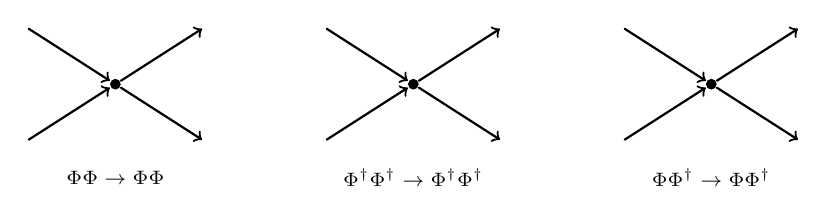
\begin{tikzpicture}[scale=0.88,line cap=round]
    \foreach \x/\lab/\a/\b/\c/\d in {0/$\Phi\Phi\to\Phi\Phi$/1/1/1/1,4.3/$\Phi^\dagger\Phi^\dagger\to\Phi^\dagger\Phi^\dagger$/-1/-1/-1/-1,8.6/$\Phi\Phi^\dagger\to\Phi\Phi^\dagger$/1/-1/1/-1}{
      \begin{scope}[xshift=\x cm]
        \fill (0,0) circle (2.2pt);
        \draw[thick,->] (-1.25,0.8)--(-0.08,0.05);
        \draw[thick,->] (-1.25,-0.8)--(-0.08,-0.05);
        \draw[thick,->] (0.08,0.05)--(1.25,0.8);
        \draw[thick,->] (0.08,-0.05)--(1.25,-0.8);
        \node[font=\scriptsize,align=center] at (0,-1.35) {\lab};
      \end{scope}
    }
  \end{tikzpicture}
  \end{center}
  树图都只有一个四点接触顶点，因此
  \[
  \boxed{\ii\mathcal M_{\rm tree}=-\ii\lambda},
  \qquad
  \boxed{\mathcal M_{\rm tree}=-\lambda},
  \]
  其中对全同粒子末态，截面计算时另按相空间规范加入 $1/2!$ 对称因子，而不改变顶点振幅本身。

  \item 一圈 1PI 图包括二点函数的 tadpole，以及四点函数中两个四点顶点组成的 bubble。四点函数有 $s,t,u$ 三种外腿配对，必须逐一保留与 $U(1)$ 荷流相容的收缩。代表性拓扑如下：
  \begin{center}
  \begin{tikzpicture}[scale=0.90,line cap=round]
    \begin{scope}[xshift=-3.0cm]
      \draw[thick,->] (-1.4,0)--(-0.05,0); \draw[thick,->] (0.05,0)--(1.4,0);
      \fill (0,0) circle (2pt);
      \draw[thick] (0,0) .. controls (-0.75,0.95) and (0.75,0.95) .. (0,0);
      \node[font=\scriptsize] at (0,-0.65) {二点 tadpole};
    \end{scope}
    \begin{scope}[xshift=2.2cm]
      \fill (-0.55,0) circle (2pt); \fill (0.55,0) circle (2pt);
      \draw[thick] (-0.55,0) arc (180:0:0.55 and 0.55);
      \draw[thick] (0.55,0) arc (0:-180:0.55 and 0.55);
      \draw[thick,->] (-1.6,0.75)--(-0.6,0.08); \draw[thick,->] (-1.6,-0.75)--(-0.6,-0.08);
      \draw[thick,->] (0.6,0.08)--(1.6,0.75); \draw[thick,->] (0.6,-0.08)--(1.6,-0.75);
      \node[font=\scriptsize] at (0,-1.0) {四点 bubble（另有 $t,u$ 通道）};
    \end{scope}
  \end{tikzpicture}
  \end{center}
  真空泡与散射振幅无关。

  二点 tadpole 与外动量无关，所以其 UV 极点只能重整化质量，不能产生 $p^2$ 反项：
  \[
  \boxed{\delta Z_\Phi^{(1)}=0}.
  \]
  直接用一个四点顶点收缩成环，得到
  \[
  \ii\Sigma_{\rm tad}
  =(-\ii\lambda)\mu^{2\epsilon}
  \int\frac{\dd[D]{\ell}}{(2\pi)^D}
  \frac{\ii}{\ell^2-m^2+\ii0}.
  \]
  其 MS 极点为 $\Sigma_{\rm div}=\lambda m^2/(16\pi^2\epsilon)$(自能 $\Sigma$ 的整体号取决于 $\ii\Gamma^{(2)}=\ii(p^2-m^2)-\ii\Sigma$ 的定义)。因此可取
  \[
  \boxed{\delta m^2=\frac{\lambda m^2}{16\pi^2}\frac1\epsilon}.
  \]

  四点函数的组合因子可不靠记忆而由实分量指标计算。令
  \[
  \Phi=\frac{\phi_1+\ii\phi_2}{\sqrt2},\qquad
  -\frac\lambda4(\Phi^\dagger\Phi)^2
  =-\frac{g}{4!}(\phi_a\phi_a)^2,
  \qquad g=\frac32\lambda.
  \]
  对 $O(N)$ 形式(最后取 $N=2$)，四点顶点为
  \[
  -\frac{\ii g}{3}T_{abcd},\qquad
  T_{abcd}=\delta_{ab}\delta_{cd}+\delta_{ac}\delta_{bd}+\delta_{ad}\delta_{bc}.
  \]
  每个 bubble 的两个内部线给出对称因子 $1/2$，而三种通道的指标收缩满足
  \[
  T_{abef}T_{efcd}+T_{acef}T_{efbd}+T_{adef}T_{efbc}
  =(N+8)T_{abcd}.
  \]
  又有
  \[
  \mu^{2\epsilon}\int\frac{\dd[D]{\ell}}{(2\pi)^D}
  \frac1{(\ell^2-m^2+\ii0)^2}\Big|_{\rm div}
  =\frac{\ii}{16\pi^2\epsilon}.
  \]
  因而一圈四点 1PI 极点为
  \[
  \ii\Gamma^{(4)}_{\rm div}
  =\frac{\ii g^2(N+8)}{288\pi^2\epsilon}T_{abcd}.
  \]
  用反项顶点 $-\ii\delta g\,T_{abcd}/3$ 消去它，得到
  \[
  \delta g=\frac{N+8}{96\pi^2}\frac{g^2}{\epsilon}.
  \]
  取 $N=2$ 并用 $g=3\lambda/2$，即
  \[
  \boxed{\delta\lambda=\frac{5\lambda^2}{32\pi^2}\frac1\epsilon}.
  \]
  裸耦合 $\lambda_0=\mu^{2\epsilon}(\lambda+\delta\lambda)$ 对 $\mu$ 不变，故
  \[
  \boxed{\beta_\lambda=-2\epsilon\lambda+\frac{5\lambda^2}{16\pi^2}+\mathcal O(\lambda^3)}.
  \]
  在严格四维极限 $\epsilon\to0$ 时只剩后一项。
\end{enumerate}
\end{solution}
\end{question}

\begin{question}[40 分]
标量 QED。
\begin{enumerate}
  \item 将第一题理论耦合到 Maxwell 场，写出标量 QED 的完整拉格朗日量密度；
  \item 在费曼规范下写出该理论所有费曼规则；
  \item 计算树图过程
  \[
  \Phi(p_1)+\Phi^*(p_2)\to\gamma(k_1)+\gamma(k_2),
  \]
  写成 $\mathcal M=\mathcal M_{\mu\nu}\epsilon^{\mu,*}(k_1)\epsilon^{\nu,*}(k_2)$，并具体检验 Ward 恒等式。
\end{enumerate}
\begin{solution}
\begin{enumerate}
  \item 取
  \[
  D_\mu=\partial_\mu+\ii eA_\mu,
  \qquad
  F_{\mu\nu}=\partial_\mu A_\nu-\partial_\nu A_\mu.
  \]
  完整规范不变拉氏量为
  \[
  \boxed{
  \mathcal L=(D_\mu\Phi)^\dagger D^\mu\Phi
  -m^2\Phi^\dagger\Phi
  -\frac\lambda4(\Phi^\dagger\Phi)^2
  -\frac14F_{\mu\nu}F^{\mu\nu}}.
  \]
  为给出费曼规范传播子，可再加入规范固定项
  \[
  \mathcal L_{\rm gf}=-\frac12(\partial_\mu A^\mu)^2.
  \]
  规范变换可取
  \[
  \Phi\to\ee^{-\ii e\alpha(x)}\Phi,
  \qquad A_\mu\to A_\mu+\partial_\mu\alpha.
  \]

  \item 费曼规范中的规则为
  \[
  \text{标量：}\quad \frac{\ii}{p^2-m^2+\ii0},
  \qquad
  \text{光子：}\quad \frac{-\ii g_{\mu\nu}}{k^2+\ii0},
  \]
  \[
  \Phi\Phi^\dagger A_\mu:\quad \boxed{\ii e(p+p')_\mu},
  \]
  \[
  \Phi\Phi^\dagger A_\mu A_\nu:\quad \boxed{2\ii e^2g_{\mu\nu}},
  \]
  \[
  \Phi^2\Phi^{\dagger2}:\quad \boxed{-\ii\lambda}.
  \]
  外部出射光子乘 $\epsilon_\mu^*(k)$；外部标量按通常 LSZ 归一化处理。

  \item 树图共有三幅：两幅标量交换图和一幅 seagull 接触图。下图中实线箭头表示带电标量，虚线表示光子：
  \begin{center}
  \begin{tikzpicture}[scale=0.86,line cap=round]
    \begin{scope}[xshift=-4.5cm]
      \fill (-0.45,0) circle (2pt); \fill (0.45,0) circle (2pt);
      \draw[thick,->] (-1.65,-0.8)--(-0.5,-0.05);
      \draw[thick,->] (1.65,-0.8)--(0.5,-0.05);
      \draw[thick,->] (-0.45,0)--(0.45,0);
      \draw[thick,dashed] (-0.45,0)--(-1.55,0.85);
      \draw[thick,dashed] (0.45,0)--(1.55,0.85);
      \node[font=\scriptsize] at (0,-1.25) {$t$ 通道};
    \end{scope}
    \begin{scope}[xshift=0cm]
      \fill (-0.45,0) circle (2pt); \fill (0.45,0) circle (2pt);
      \draw[thick,->] (-1.65,-0.8)--(-0.5,-0.05);
      \draw[thick,->] (1.65,-0.8)--(0.5,-0.05);
      \draw[thick,->] (-0.45,0)--(0.45,0);
      \draw[thick,dashed] (-0.45,0)--(1.55,0.85);
      \draw[thick,dashed] (0.45,0)--(-1.55,0.85);
      \node[font=\scriptsize] at (0,-1.25) {$u$ 通道};
    \end{scope}
    \begin{scope}[xshift=4.5cm]
      \fill (0,0) circle (2.4pt);
      \draw[thick,->] (-1.55,-0.8)--(-0.08,-0.04);
      \draw[thick,->] (1.55,-0.8)--(0.08,-0.04);
      \draw[thick,dashed] (0,0)--(-1.45,0.85);
      \draw[thick,dashed] (0,0)--(1.45,0.85);
      \node[font=\scriptsize] at (0,-1.25) {seagull};
    \end{scope}
  \end{tikzpicture}
  \end{center}
  令
  \[
  D_t=(p_1-k_1)^2-m^2,
  \qquad
  D_u=(p_1-k_2)^2-m^2.
  \]
  则可取
  \[
  \boxed{
  \mathcal M_{\mu\nu}=e^2\left[
  2g_{\mu\nu}
  +\frac{(2p_1-k_1)_\mu(2p_2-k_2)_\nu}{D_t}
  +\frac{(2p_2-k_1)_\mu(2p_1-k_2)_\nu}{D_u}
  \right]}.
  \]
  于是
  \[
  \mathcal M=\mathcal M_{\mu\nu}\epsilon^{\mu,*}(k_1)\epsilon^{\nu,*}(k_2).
  \]
  用 $p_i^2=m^2$、$k_i^2=0$ 与 $p_1+p_2=k_1+k_2$，有
  \[
  D_t=-2p_1\cdot k_1,
  \qquad D_u=-2p_2\cdot k_1,
  \]
  因而
  \[
  \begin{aligned}
  k_1^\mu\mathcal M_{\mu\nu}/e^2
  &=2k_{1\nu}-(2p_2-k_2)_\nu-(2p_1-k_2)_\nu\\
  &=2[k_1-(p_1+p_2-k_2)]_\nu=0.
  \end{aligned}
  \]
  同理 $k_2^\nu\mathcal M_{\mu\nu}=0$。故
  \[
  \boxed{k_1^\mu\mathcal M_{\mu\nu}=0,
  \qquad k_2^\nu\mathcal M_{\mu\nu}=0},
  \]
  即树图振幅满足 Ward 恒等式；seagull 图正是保证上述相消所必需的项。
\end{enumerate}
\end{solution}
\end{question}

\begin{question}[20 分]
考虑模型
\[
\mathcal L=\frac12(\partial_\mu\sigma)^2
+\ii\sum_{j=1}^{N_f}\bar\psi_j\not{\partial}\psi_j
-\sum_{j=1}^{N_f}g_1\sigma\bar\psi_j\psi_j
-\frac1{4!}g_2\sigma^4,
\]
其中 $\sigma$ 为实标量场，$\psi_j$($j=1,\ldots,N_f$)为 $N_f$ 个狄拉克场。采用维数正规化 $D=4-2\epsilon$ 和 MS 方案。
\begin{enumerate}
  \item 定义重整化场 $\sigma=\sqrt{Z_\sigma}\sigma_r$、$\psi_j=\sqrt{Z_\psi}\psi_{r,j}$ 和重整化耦合
  \[
  g_1=\mu^\epsilon Z_1g_{r,1},\qquad
  g_2=\mu^{2\epsilon}Z_2g_{r,2}.
  \]
  写出重整化微扰论下的拉格朗日密度及所有费曼规则(含抵消项)；
  \item 计算单圈场重整化常数；
  \item 计算 $g_{r,1}^2$ 和 $g_{r,2}$ 的单圈 beta 函数；
  \item 利用 $4-2\epsilon$ 展开，取 $N_f=1/4$，尽可能找出 $g_{r,2}>0$ 的 beta 函数零点并判断红外稳定性，在 $g_{r,1}^2-g_{r,2}$ 平面画出 RG 流。
\end{enumerate}
\begin{solution}
下文把 $g_{r,1},g_{r,2}$ 简记为 $g_1,g_2$。
\begin{enumerate}
  \item 代入场与耦合重整化后
  \[
  \begin{aligned}
  \mathcal L={}&\frac12Z_\sigma(\partial\sigma_r)^2
  +\ii Z_\psi\sum_{j=1}^{N_f}\bar\psi_{r,j}\not{\partial}\psi_{r,j}\\
  &-\mu^\epsilon Z_1Z_\psi Z_\sigma^{1/2}g_1
  \sigma_r\sum_j\bar\psi_{r,j}\psi_{r,j}
  -\frac{\mu^{2\epsilon}}{4!}Z_2Z_\sigma^2g_2\sigma_r^4.
  \end{aligned}
  \]
  写 $Z_a=1+\delta Z_a$ 后，可分成重整化自由部分、重整化相互作用与抵消项。树级规则为
  \[
  \sigma:\quad \frac{\ii}{p^2+\ii0},
  \qquad
  \psi:\quad \frac{\ii\not p}{p^2+\ii0},
  \]
  \[
  \sigma\bar\psi\psi:\quad -\ii\mu^\epsilon g_1,
  \qquad
  \sigma^4:\quad -\ii\mu^{2\epsilon}g_2.
  \]
  对应抵消项规则为
  \[
  \sigma\text{ 二点}:\quad \ii\delta Z_\sigma p^2,
  \qquad
  \psi\text{ 二点}:\quad \ii\delta Z_\psi\not p,
  \]
  \[
  \sigma\bar\psi\psi:\quad
  -\ii\mu^\epsilon g_1
  \left(\delta Z_1+\delta Z_\psi+\frac12\delta Z_\sigma\right),
  \]
  \[
  \sigma^4:\quad
  -\ii\mu^{2\epsilon}g_2
  \left(\delta Z_2+2\delta Z_\sigma\right).
  \]

  \item 费米子自能的一圈图含一条 $\sigma$ 与一条费米子传播线；标量自能的一圈图为闭合费米子环。只取 $p^2$ 或 $\not p$ 的 UV 极点，得到
  \[
  \boxed{Z_\psi=1-\frac{g_1^2}{32\pi^2\epsilon}+\mathcal O(g^4)},
  \]
  \[
  \boxed{Z_\sigma=1-\frac{N_f g_1^2}{8\pi^2\epsilon}+\mathcal O(g^4)}.
  \]
  第二式中的 $4N_f$ 来自四分量 Dirac 自旋迹。$\sigma^4$ tadpole 在无质量维数正规化中为无标度积分，不产生一圈波函数重整化。

  为后续 beta 函数，MS 下还可写出完整耦合重整化的单极点：
  \[
  Z_1=1+\frac{(2N_f+3)g_1^2}{32\pi^2\epsilon}+\mathcal O(g^4),
  \]
  以及更适合在 $g_2\to0$ 时使用的加性形式
  \[
  g_{2,0}=\mu^{2\epsilon}\left[g_2+\frac{3g_2^2+8N_fg_1^2g_2-48N_fg_1^4}{32\pi^2\epsilon}\right].
  \]

  \item 由裸耦合对 $\mu$ 不变，得到
  \[
  \boxed{
  \beta_{g_1^2}\equiv\mu\frac{\dd{g_1^2}}{\dd\mu}
  =-2\epsilon g_1^2
  +\frac{2N_f+3}{8\pi^2}g_1^4},
  \]
  \[
  \boxed{
  \beta_{g_2}\equiv\mu\frac{\dd{g_2}}{\dd\mu}
  =-2\epsilon g_2
  +\frac{3g_2^2+8N_fg_1^2g_2-48N_fg_1^4}{16\pi^2}}.
  \]
  当把维数写成常见的 $d=4-\varepsilon$ 时，只需令 $\varepsilon=2\epsilon$，即得到标准 chiral-Ising Gross--Neveu--Yukawa 的一圈流方程。

  \item 取
  \[
  x=g_1^2,\qquad y=g_2,\qquad N_f=\frac14.
  \]
  则
  \[
  \beta_x=-2\epsilon x+\frac{7}{16\pi^2}x^2,
  \]
  \[
  \beta_y=-2\epsilon y+\frac{3y^2+2xy-12x^2}{16\pi^2}.
  \]
  第一式给
  \[
  x=0\quad\text{或}\quad x=\frac{32\pi^2}{7}\epsilon.
  \]
  当 $x=0$ 时，$\beta_y=0$ 给出
  \[
  (x,y)=(0,0),\qquad
  \boxed{P_{\rm WF}=\left(0,\frac{32\pi^2}{3}\epsilon\right)}.
  \]
  当 $x=32\pi^2\epsilon/7$ 时，令 $y=c\pi^2\epsilon$，得到
  \[
  147c^2-1120c-12288=0,
  \]
  即
  \[
  c=\frac{96}{7}\quad\text{或}\quad c=-\frac{128}{21}.
  \]
  因此 $y>0$ 的相互作用零点为
  \[
  \boxed{P_{\rm GNY}=\left(
  \frac{32\pi^2}{7}\epsilon,
  \frac{96\pi^2}{7}\epsilon\right)}.
  \]
  另一个 Yukawa 零点具有 $y<0$，四次势不稳定，按题目要求舍去。

  真正的红外稳定性还要检查稳定矩阵 $J_{ij}=\partial\beta_i/\partial g_j$。在 $P_{\rm GNY}$，
  \[
  J=\epsilon\begin{pmatrix}
  2&0\\[-1mm]
  -36/7&26/7
  \end{pmatrix},
  \]
  本征值为
  \[
  \boxed{2\epsilon,\quad \frac{26}{7}\epsilon>0}.
  \]
  因为红外对应 $\ln\mu\to-\infty$，正本征值意味着扰动衰减，所以 $P_{\rm GNY}$ 是完全 IR 吸引的固定点。$P_{\rm WF}$ 虽满足 $y>0$，但沿 Yukawa 方向有
  \[
  \left.\frac{\partial\beta_x}{\partial x}\right|_{P_{\rm WF}}=-2\epsilon<0,
  \]
  因此它只是鞍点，Yukawa 耦合是其红外相关方向。

  \begin{center}
  \begin{tikzpicture}[>=stealth,x=1cm,y=1cm,scale=1.18]
    % Coordinates: X=x/(pi^2 epsilon), Y=y/(pi^2 epsilon).
    \draw[->,thick] (0,0)--(7.15,0) node[right,font=\small] {$x/(\pi^2\epsilon)$};
    \draw[->,thick] (0,0)--(0,7.05) node[above,font=\small] {$y/(\pi^2\epsilon)$};
    \foreach \X in {1,2,3,4,5,6}{
      \draw (1.15*\X,0.07)--(1.15*\X,-0.07) node[below,font=\small] {\X};
    }
    \foreach \Y in {4,8,12,16}{
      \draw (0.07,0.42*\Y)--(-0.07,0.42*\Y) node[left,font=\small] {\Y};
    }
  \draw[->,thick] (0.690,0.630) -- ++(0.100,0.262);
  \draw[->,thick] (0.690,1.806) -- ++(0.056,0.274);
  \draw[->,thick] (0.690,2.982) -- ++(0.063,0.273);
  \draw[->,thick] (0.690,4.158) -- ++(0.207,0.189);
  \draw[->,thick] (0.690,5.334) -- ++(0.052,-0.275);
  \draw[->,thick] (0.690,6.384) -- ++(0.021,-0.279);
  \draw[->,thick] (1.955,0.630) -- ++(0.122,0.252);
  \draw[->,thick] (1.955,1.806) -- ++(0.089,0.266);
  \draw[->,thick] (1.955,2.982) -- ++(0.103,0.260);
  \draw[->,thick] (1.955,4.158) -- ++(0.230,0.160);
  \draw[->,thick] (1.955,5.334) -- ++(0.103,-0.260);
  \draw[->,thick] (1.955,6.384) -- ++(0.042,-0.277);
  \draw[->,thick] (3.220,0.630) -- ++(0.074,0.270);
  \draw[->,thick] (3.220,1.806) -- ++(0.062,0.273);
  \draw[->,thick] (3.220,2.982) -- ++(0.072,0.271);
  \draw[->,thick] (3.220,4.158) -- ++(0.138,0.244);
  \draw[->,thick] (3.220,5.334) -- ++(0.150,-0.236);
  \draw[->,thick] (3.220,6.384) -- ++(0.048,-0.276);
  \draw[->,thick] (4.485,0.630) -- ++(0.024,0.279);
  \draw[->,thick] (4.485,1.806) -- ++(0.022,0.279);
  \draw[->,thick] (4.485,2.982) -- ++(0.025,0.279);
  \draw[->,thick] (4.485,4.158) -- ++(0.040,0.277);
  \draw[->,thick] (4.485,5.334) -- ++(0.266,0.087);
  \draw[->,thick] (4.485,6.384) -- ++(0.036,-0.278);
  \draw[->,thick] (5.750,0.630) -- ++(-0.013,0.280);
  \draw[->,thick] (5.750,1.806) -- ++(-0.012,0.280);
  \draw[->,thick] (5.750,2.982) -- ++(-0.014,0.280);
  \draw[->,thick] (5.750,4.158) -- ++(-0.019,0.279);
  \draw[->,thick] (5.750,5.334) -- ++(-0.043,0.277);
  \draw[->,thick] (5.750,6.384) -- ++(-0.069,-0.271);
  \draw[->,thick] (6.670,0.630) -- ++(-0.032,0.278);
  \draw[->,thick] (6.670,1.806) -- ++(-0.032,0.278);
  \draw[->,thick] (6.670,2.982) -- ++(-0.035,0.278);
  \draw[->,thick] (6.670,4.158) -- ++(-0.044,0.276);
  \draw[->,thick] (6.670,5.334) -- ++(-0.075,0.270);
  \draw[->,thick] (6.670,6.384) -- ++(-0.259,0.107);
    \fill (0,0) circle (2.0pt);
    \node[below right=2pt,font=\small] at (0,0) {$G$};
    \fill (0,{0.42*32/3}) circle (2.3pt);
    \node[left=4pt,font=\small,fill=white,inner sep=1pt] at (0,{0.42*32/3}) {$P_{\rm WF}$};
    \fill ({1.15*32/7},{0.42*96/7}) circle (2.3pt);
    \node[above right=3pt,font=\small,fill=white,inner sep=1pt] at ({1.15*32/7},{0.42*96/7}) {$P_{\rm GNY}$};
    \node[font=\small,align=center] at (4.9,0.65) {箭头指向低能\\($\mu\downarrow$)};
  \end{tikzpicture}
  \par\smallskip
  {\small $N_f=1/4$ 时的红外 RG 流。固定点标签与流线分离，便于辨认。}
  \end{center}
\end{enumerate}
\end{solution}
\end{question}

\clearpage
\begin{center}
{\Large\bfseries 原卷附：2025 PKU QFT-1 Cheat Sheet}
\end{center}
\footnotesize
\begin{multicols}{2}
\textbf{Free real scalar field}

\[
\mathcal L=\frac12\partial_\mu\phi\partial^\mu\phi-\frac12m^2\phi^2.
\]
\[
\phi(x)=\int\frac{\dd[3]{p}}{(2\pi)^3\,2E_{\mathbf p}}
\left(a_{\mathbf p}\ee^{-\ii p\cdot x}+a_{\mathbf p}^\dagger\ee^{\ii p\cdot x}\right).
\]
\[
[a_{\mathbf p},a_{\mathbf p'}^\dagger]=(2\pi)^3 2E_{\mathbf p}\delta^{(3)}(\mathbf p-\mathbf p').
\]
\[
a_{\mathbf p}|0\rangle=0,
\qquad |\mathbf p\rangle=a_{\mathbf p}^\dagger|0\rangle.
\]
若无穷小变换 $\phi\to\phi+\epsilon\delta\phi$ 使
$\mathcal L\to\mathcal L+\epsilon\partial_\mu F^\mu$，则
\[
j^\mu=\frac{\partial\mathcal L}{\partial(\partial_\mu\phi)}\delta\phi-F^\mu.
\]
平移对称给出
\[
T^{\mu\nu}=\frac{\partial\mathcal L}{\partial(\partial_\mu\phi)}\partial^\nu\phi-g^{\mu\nu}\mathcal L,
\qquad
P^\mu=\int\dd[3]{x}\,T^{0\mu}=(H,\mathbf P).
\]
\[
H=\int\frac{\dd[3]{p}}{(2\pi)^3\,2E_{\mathbf p}}
E_{\mathbf p}a_{\mathbf p}^\dagger a_{\mathbf p},
\quad
\mathbf P=\int\frac{\dd[3]{p}}{(2\pi)^3\,2E_{\mathbf p}}
\mathbf p\,a_{\mathbf p}^\dagger a_{\mathbf p}.
\]
\[
[P^\mu,\phi(x)]=-\ii\partial^\mu\phi(x),
\qquad \phi(x)=\ee^{\ii P\cdot x}\phi(0)\ee^{-\ii P\cdot x}.
\]
Lorentz 流与荷：
\[
\mathcal J^{\mu,\rho\sigma}=x^\rho T^{\mu\sigma}-x^\sigma T^{\mu\rho},
\qquad
J^{\rho\sigma}=\int\dd[3]{x}\,\mathcal J^{0,\rho\sigma}.
\]
\[
\langle0|T\phi(x)\phi(y)|0\rangle
=\int\frac{\dd[4]{p}}{(2\pi)^4}\frac{\ii\ee^{-\ii p\cdot(x-y)}}{p^2-m^2+\ii\epsilon}.
\]
Wick 定理示例：四场时间序乘积等于正常序项加所有单收缩与双收缩项。

\columnbreak
\textbf{Free Dirac field}

\[
\{\gamma^\mu,\gamma^\nu\}=2g^{\mu\nu}I.
\]
Weyl 基：
\[
\gamma^\mu=\begin{pmatrix}0&\sigma^\mu\\\bar\sigma^\mu&0\end{pmatrix},
\quad
\sigma^\mu=(I,\boldsymbol\sigma),
\quad
\bar\sigma^\mu=(I,-\boldsymbol\sigma).
\]
\[
\mathcal L=\bar\psi(\ii\not\partial-m)\psi,
\qquad \bar\psi=\psi^\dagger\gamma^0.
\]
\[
(\ii\not\partial-m)\psi=0,
\qquad
\bar\psi(\ii\overleftarrow{\not\partial}+m)=0.
\]
\[
\psi(x)=\int\frac{\dd[3]{p}}{(2\pi)^3\,2E_{\mathbf p}}
\sum_s\left(a_{\mathbf p}^s u^s(p)\ee^{-\ii p\cdot x}
+b_{\mathbf p}^{s\dagger}v^s(p)\ee^{\ii p\cdot x}\right).
\]
\[
\{a_{\mathbf p}^r,a_{\mathbf q}^{s\dagger}\}
=\{b_{\mathbf p}^r,b_{\mathbf q}^{s\dagger}\}
=(2\pi)^3\delta^{rs}2E_{\mathbf p}\delta^{(3)}(\mathbf p-\mathbf q).
\]
\[
a_{\mathbf p}^s|0\rangle=b_{\mathbf p}^s|0\rangle=0,
\quad
|p,a,s\rangle=a_{\mathbf p}^{s\dagger}|0\rangle,
\quad
|p,b,s\rangle=b_{\mathbf p}^{s\dagger}|0\rangle.
\]
\[
\sum_su^s(p)\bar u^s(p)=\not p+m,
\qquad
\sum_sv^s(p)\bar v^s(p)=\not p-m.
\]
\[
\bar u^s(p)u^r(p)=2m\delta^{sr},
\qquad
\bar v^s(p)v^r(p)=-2m\delta^{sr}.
\]
\[
u^{s\dagger}(p)u^r(p)=v^{s\dagger}(p)v^r(p)=2E_p\delta^{sr}.
\]
\[
T^{\mu\nu}=\ii\bar\psi\gamma^\mu\partial^\nu\psi-g^{\mu\nu}\mathcal L.
\]
\[
H=\int\frac{\dd[3]{p}}{(2\pi)^3\,2E_p}E_p
\sum_s(a_{\mathbf p}^{s\dagger}a_{\mathbf p}^s+b_{\mathbf p}^{s\dagger}b_{\mathbf p}^s).
\]
\[
J^{\mu,\alpha\beta}=x^\alpha T^{\mu\beta}-x^\beta T^{\mu\alpha}
+\bar\psi\gamma^\mu\Sigma^{\alpha\beta}\psi,
\qquad
\Sigma^{\mu\nu}=\frac\ii4[\gamma^\mu,\gamma^\nu].
\]
\[
j^\mu=\bar\psi\gamma^\mu\psi,
\qquad Q=\int\dd[3]{x}\,j^0,
\]
\[
Q=\int\frac{\dd[3]{p}}{(2\pi)^3\,2E_p}\sum_s
\left(a_{\mathbf p}^{s\dagger}a_{\mathbf p}^s
-b_{\mathbf p}^{s\dagger}b_{\mathbf p}^s\right).
\]
\[
\partial_\mu T^{\mu\nu}=0,\qquad
\partial_\mu J^{\mu,\alpha\beta}=0,\qquad
\partial_\mu j^\mu=0.
\]
\[
S_F(x-y)=\int\frac{\dd[4]{p}}{(2\pi)^4}
\frac{\ii(\not p+m)}{p^2-m^2+\ii\epsilon}\ee^{-\ii p\cdot(x-y)}.
\]

\columnbreak
\textbf{Free $U(1)$ gauge field, Feynman gauge}

\[
\mathcal L=-\frac14F_{\mu\nu}F^{\mu\nu}-\frac12(\partial_\mu A^\mu)^2,
\quad
F_{\mu\nu}=\partial_\mu A_\nu-\partial_\nu A_\mu.
\]
\[
\partial_\mu F^{\mu\nu}+\partial^\nu(\partial\cdot A)=0.
\]
\[
A^\mu(x)=\int\frac{\dd[3]{p}}{(2\pi)^3\,2E_p}
\sum_{\lambda=0}^3\epsilon_\lambda^\mu(p)
\left(a_{\mathbf p}^\lambda\ee^{-\ii p\cdot x}+a_{\mathbf p}^{\lambda\dagger}\ee^{\ii p\cdot x}\right).
\]
\[
[a_{\mathbf p}^\lambda,a_{\mathbf q}^{\sigma\dagger}]
=-(2\pi)^3 2E_p\delta^{(3)}(\mathbf p-\mathbf q)g^{\lambda\sigma}.
\]
\[
\sum_{\lambda=0}^3\epsilon_\lambda^\mu(p)\epsilon_\lambda^{\nu*}(p)=-g^{\mu\nu}.
\]
\[
D_{\mu\nu}(p)=\frac{-\ii g_{\mu\nu}}{p^2+\ii\epsilon}.
\]
\[
\langle0|T A_\mu(x)A_\nu(y)|0\rangle
=\int\frac{\dd[4]{p}}{(2\pi)^4}D_{\mu\nu}(p)\ee^{-\ii p\cdot(x-y)}.
\]
\end{multicols}

\begin{multicols}{2}
\textbf{Discrete symmetry}

Parity $P:(t,\mathbf x)\mapsto(t,-\mathbf x)$：
\[
\phi(t,\mathbf x)\to\phi(t,-\mathbf x)\quad\text{(scalar)},
\]
\[
\phi(t,\mathbf x)\to-\phi(t,-\mathbf x)\quad\text{(pseudoscalar)},
\]
\[
\psi(x)\to\eta_P\gamma^0\psi(Px),\qquad
A^\mu\to(A^0,-\mathbf A)(Px).
\]
Time reversal $T:(t,\mathbf x)\mapsto(-t,\mathbf x)$：
\[
\phi(t,\mathbf x)\to\phi(-t,\mathbf x),
\qquad
A^\mu\to(A^0,-\mathbf A)(Tx),
\]
并对自旋场使用相应反幺正变换。

Charge conjugation：
\[
\phi(x)\to\phi^\dagger(x),
\qquad
\psi(x)\to-\ii\gamma^2\psi^*(x),
\qquad
A^\mu\to-A^\mu.
\]

\textbf{Interacting real scalar field}

\[
\mathcal L=\frac12(\partial\phi_0)^2-\frac12m_0^2\phi_0^2-\frac{\lambda_0}{4!}\phi_0^4.
\]
\[
\phi_0=\sqrt{Z_\phi}\phi,
\qquad m_0^2=Z_m m^2,
\qquad \lambda_0=Z_\lambda\lambda\mu^{2\epsilon}.
\]
\[
\begin{aligned}
\mathcal L={}&\frac12(\partial\phi)^2-\frac12m^2\phi^2-\frac{\lambda\mu^{2\epsilon}}{4!}\phi^4\\
&+\frac12\delta_Z(\partial\phi)^2-\frac12\delta_m m^2\phi^2
-\delta_\lambda\frac{\lambda\mu^{2\epsilon}}{4!}\phi^4.
\end{aligned}
\]
反项规则：外线标量 $1$；$\phi^4$ 顶点 $-\ii\lambda\mu^{2\epsilon}$；自能反项 $\ii(\delta_Zp^2-\delta_m m^2)$；顶点反项 $-\ii\delta_\lambda\lambda\mu^{2\epsilon}$。

\columnbreak
\textbf{Quantum Electrodynamics}

忽略规范固定项时的裸拉氏量：
\[
\mathcal L=-\frac14(F_{0,\mu\nu})^2+\bar\psi_0(\ii\not\partial-m_0)\psi_0
-e_0\bar\psi_0\not A_0\psi_0.
\]
\[
\psi_0=\sqrt{Z_2}\psi,\qquad
A_0^\mu=\sqrt{Z_3}A^\mu,
\]
\[
m_0=Z_m m,\qquad
e_0=\frac{Z_1}{Z_2\sqrt{Z_3}}e.
\]
费曼规则：
\begin{itemize}
\item 入/出电子：$u(p),\bar u(p)$；
\item 入/出正电子：$\bar v(p),v(p)$；
\item 入/出光子：$\epsilon_\mu(p),\epsilon_\mu^*(p)$；
\item 顶点：$-\ii e\mu^\epsilon\gamma^\mu$；
\item 电子自能反项：$\ii(\delta_2\not p-\delta_m m)$；
\item 光子自能反项：$-\ii(g^{\mu\nu}p^2-p^\mu p^\nu)\delta_3$；
\item 顶点反项：$-\ii e\mu^\epsilon\gamma^\mu\delta_1$。
\end{itemize}
其中 $\delta_i=Z_i-1$，$\delta_m=Z_2Z_m-1$。

\textbf{Spinor helicity, massless}

\[
|i^\pm\rangle\equiv|k_i^\pm\rangle
=u_\pm(k_i)=v_\mp(k_i),
\]
\[
\langle i^\pm|\equiv\langle k_i^\pm|
=\bar u_\pm(k_i)=\bar v_\mp(k_i).
\]
\[
\langle ij\rangle=\bar u_-(k_i)u_+(k_j),
\qquad
[ij]=\bar u_+(k_i)u_-(k_j).
\]
\[
\langle ij\rangle[ij]=2k_i\cdot k_j=s_{ij},
\qquad
\langle ij\rangle=-\langle ji\rangle,
\qquad [ij]=-[ji].
\]
\[
\langle i^\pm|\gamma^\mu|i^\pm\rangle=2k_i^\mu,
\qquad
|i^\pm\rangle\langle i^\pm|=\frac12(1\pm\gamma^5)\not k_i.
\]
\[
[i|\gamma^\mu|j\rangle\,[k|\gamma_\mu|l\rangle
=2[ik]\langle lj\rangle,
\]
\[
[i|\gamma^\mu|j\rangle=\langle j|\gamma^\mu|i],
\qquad
\langle ij\rangle\langle kl\rangle
=\langle ik\rangle\langle jl\rangle+\langle il\rangle\langle kj\rangle.
\]
原卷以参考无质量动量 $r$ 给出的光子极化矢量为
\[
\epsilon_+^{*,\mu}(k,r)
=-\frac{\langle r|\gamma^\mu|k]}{\sqrt2\langle rk\rangle},
\qquad
\epsilon_-^{*,\mu}(k,r)
=-\frac{[r|\gamma^\mu|k\rangle}{\sqrt2[rk]}.
\]

\columnbreak
\textbf{Useful formulae}

\[
\frac1{A_1\cdots A_n}
=\int_0^1\dd{x_1}\cdots\dd{x_n}\,
\frac{\delta(\sum_i x_i-1)(n-1)!}
{(x_1A_1+\cdots+x_nA_n)^n}.
\]
\[
\int\frac{\dd[d]{\ell}}{(2\pi)^d}\frac1{(\ell^2-\Delta)^n}
=\frac{(-1)^n\ii}{(4\pi)^{d/2}}
\frac{\Gamma(n-d/2)}{\Gamma(n)}
\left(\frac1\Delta\right)^{n-d/2}.
\]
\[
\begin{aligned}
&\int\frac{\dd[d]{\ell}}{(2\pi)^d}
\frac{\ell^2}{(\ell^2-\Delta)^n}\\
&\quad=\frac{(-1)^{n-1}\ii}{(4\pi)^{d/2}}\frac d2
\frac{\Gamma(n-d/2-1)}{\Gamma(n)}
\left(\frac1\Delta\right)^{n-d/2-1}.
\end{aligned}
\]
\[
\begin{aligned}
&\int\frac{\dd[d]{\ell}}{(2\pi)^d}
\frac{\ell^\mu\ell^\nu}{(\ell^2-\Delta)^n}\\
&\quad=\frac{(-1)^{n-1}\ii}{(4\pi)^{d/2}}\frac{g^{\mu\nu}}2
\frac{\Gamma(n-d/2-1)}{\Gamma(n)}
\left(\frac1\Delta\right)^{n-d/2-1}.
\end{aligned}
\]
\[
\begin{aligned}
&\int\frac{\dd[d]{\ell}}{(2\pi)^d}
\frac{(\ell^2)^2}{(\ell^2-\Delta)^n}\\
&\quad=\frac{(-1)^n\ii}{(4\pi)^{d/2}}\frac{d(d+2)}4
\frac{\Gamma(n-d/2-2)}{\Gamma(n)}
\left(\frac1\Delta\right)^{n-d/2-2}.
\end{aligned}
\]
\[
\begin{aligned}
&\int\frac{\dd[d]{\ell}}{(2\pi)^d}
\frac{\ell^\mu\ell^\nu\ell^\rho\ell^\sigma}{(\ell^2-\Delta)^n}\\
&=\frac{(-1)^n\ii}{(4\pi)^{d/2}}
\frac{\Gamma(n-d/2-2)}{\Gamma(n)}
\left(\frac1\Delta\right)^{n-d/2-2}\\
&\quad\times\frac14\bigl(g^{\mu\nu}g^{\rho\sigma}
+g^{\mu\rho}g^{\nu\sigma}+g^{\mu\sigma}g^{\nu\rho}\bigr).
\end{aligned}
\]
\[
\Gamma(\epsilon)=\frac1\epsilon-\gamma+\mathcal O(\epsilon).
\]

两体无质量散射：
\[
\frac{\dd\sigma}{\dd t}=\frac{|\mathcal M|^2}{16\pi s^2},
\]
\[
s=(p_1+p_2)^2,\qquad t=(p_1-k_1)^2,\qquad u=(p_1-k_2)^2.
\]
一般衰变率：
\[
\dd\Gamma=\frac1{2m_A}\left(\prod_f\frac{\dd[3]{p_f}}{(2\pi)^3 2E_f}\right)
|\mathcal M|^2(2\pi)^4\delta^{(4)}\!\left(p_A-\sum_fp_f\right).
\]
Gamma 矩阵：
\[
\operatorname{tr}(\gamma^\mu\gamma^\nu)=4g^{\mu\nu},
\]
\[
\operatorname{tr}(\gamma^\mu\gamma^\nu\gamma^\rho\gamma^\sigma)
=4(g^{\mu\nu}g^{\rho\sigma}-g^{\mu\rho}g^{\nu\sigma}+g^{\mu\sigma}g^{\nu\rho}),
\]
\[
\operatorname{tr}(\gamma^\mu\gamma^\nu\gamma^\rho\gamma^\sigma\gamma^5)
=-4\ii\epsilon^{\mu\nu\rho\sigma},
\]
\[
\gamma^\mu\gamma_\mu=4,
\qquad
\gamma^\mu\gamma^\nu\gamma_\mu=-2\gamma^\nu,
\qquad
\gamma^\mu\gamma^\nu\gamma^\rho\gamma_\mu=4g^{\nu\rho},
\]
\[
\gamma^\mu\gamma^\nu\gamma^\rho\gamma^\sigma\gamma_\mu
=-2\gamma^\sigma\gamma^\rho\gamma^\nu.
\]
\end{multicols}
\normalsize
